%%%%%%%%%%%%%%%%%%%%%%%%%%%%%%%%%%%%%%%%%
% Short Sectioned Assignment
% LaTeX Template
% Version 1.0 (5/5/12)
%
% This template has been downloaded from:
% http://www.LaTeXTemplates.com
%
% Original author:
% Frits Wenneker (http://www.howtotex.com)
%
% License:
% CC BY-NC-SA 3.0 (http://creativecommons.org/licenses/by-nc-sa/3.0/)
%
%%%%%%%%%%%%%%%%%%%%%%%%%%%%%%%%%%%%%%%%%

%----------------------------------------------------------------------------
%	PACKAGES AND OTHER DOCUMENT CONFIGURATIONS
%----------------------------------------------------------------------------

\documentclass[paper=a4, fontsize=11pt]{scrartcl} % A4 paper and 11pt font size

\usepackage[T1]{fontenc} % Use 8-bit encoding that has 256 glyphs
\usepackage{fourier} % Use the Adobe Utopia font for the document - comment this line to return to the LaTeX default
\usepackage[english]{babel} % English language/hyphenation
\usepackage{amsmath,amsfonts,amsthm} % Math packages

\usepackage{lipsum} % Used for inserting dummy 'Lorem ipsum' text into the template

\usepackage{graphicx} % Used for including graphics
\usepackage{caption}
\usepackage{subcaption}

\usepackage{sectsty} % Allows customizing section commands
\allsectionsfont{\centering \normalfont\scshape} % Make all sections centered, the default font and small caps

\usepackage{fancyhdr} % Custom headers and footers
\usepackage{cite}
\bibliographystyle{plain}
\pagestyle{fancyplain} % Makes all pages in the document conform to the custom headers and footers
\fancyhead{} % No page header - if you want one, create it in the same way as the footers below
\fancyfoot[L]{} % Empty left footer
\fancyfoot[C]{} % Empty center footer
\fancyfoot[R]{\thepage} % Page numbering for right footer
\renewcommand{\headrulewidth}{0pt} % Remove header underlines
\renewcommand{\footrulewidth}{0pt} % Remove footer underlines
\setlength{\headheight}{13.6pt} % Customize the height of the header

\numberwithin{equation}{section} % Number equations within sections (i.e. 1.1, 1.2, 2.1, 2.2 instead of 1, 2, 3, 4)
\numberwithin{figure}{section} % Number figures within sections (i.e. 1.1, 1.2, 2.1, 2.2 instead of 1, 2, 3, 4)
\numberwithin{table}{section} % Number tables within sections (i.e. 1.1, 1.2, 2.1, 2.2 instead of 1, 2, 3, 4)

\setlength\parindent{0pt} % Removes all indentation from paragraphs - comment this line for an assignment with lots of text

%----------------------------------------------------------------------------
%	TITLE SECTION
%----------------------------------------------------------------------------

\newcommand{\horrule}[1]{\rule{\linewidth}{#1}} % Create horizontal rule command with 1 argument of height

\title{
\normalfont \normalsize
\textsc{King Abdullah University of Science and Technology\\
        Division of Mathematical and Computer Sciences and Engineering\\
        Design and Analysis of Algorithms} \\ [25pt] % Your university, school and/or department name(s)
\horrule{0.5pt} \\[0.4cm] % Thin top horizontal rule
\Large Midterm Project Report\\
\huge Diverse Approaches to Exact Pattern Matching
\horrule{2pt} \\[0.5cm] % Thick bottom horizontal rule
}

\author{Affara, Lama\\
        Almansour, Durrah\\
        Al-Shedivat, Maruan\\
        Chen, Gui\\
        Fujii, Chisato\\
        Rapakoulia, Trisevgeni}


\date{\normalsize\today} % Today's date or a custom date


\begin{document}
\begin{titlepage}
\maketitle
\thispagestyle{empty}
\clearpage
\end{titlepage}

%----------------------------------------------------------------------------
%    INTRODUCTION
%----------------------------------------------------------------------------

\section{Introduction}
Write introduction here

\section{Boyre Moore}
Boyre Moore algorithm \cite{bm_fast} searches for all the occurrences of the pattern in the text. It is in some way similar to the naive search algorithm. Initially, it aligns the first character in P with the first character in T. The algorithm then compares characters between P and T sequentially from right to left. Once a mismatch occurs, a shift rule is applied thus moving the pattern by $s\ge 1$. The algorithm is basically divided into two stages: preprocessing and searching. There are two different preprocessing approaches in the literature: Bad Character Rule and Good Suffix Tree \cite{bm_tbc}. We decided to choose the Bad Character rule due to its simplicity and applicability to our dataset. In the following sections, we describe the two stages of the algorithm.

\subsection{Preprocessing Stage}
In the preprocessing stage, the algorithm makes use of the alphabet $\Sigma$ and the pattern P. A two dimensional table D is constructed by processing the pattern according to the available alphabet. D is of size $k\times|\Sigma|$ where for each mismatch index in P, the position of rightmost occurrence of a character in $\Sigma$ is stored. Figure \ref{table} shows an example of the table stored by processing the pattern GCAGAGAG based on the DNA alphabet=\{A,C,G,T\}. Starting from the last row corresponding to a mismatch occurring at position i=k in P, i=8 for this example, the algorithm scans P to find the rightmost index of the given character. In the below example, the last occurrence of A before position 8 is 7, G is 6, C is 2, and T is 0. It is important to note here that if a character does not exist in the pattern, its position in the table is always 0. Now, the algorithm iterates from i=k to 1. If the mismatch occurs in position i-1, the algorithm updates only the value for the specific character placed in this position, A for this example, and all the other values remain the same as D[i,x]. The last occurrence of A before position 7 is 5, while G, C, and T stay the same.

\begin{figure}[h!]
\centering
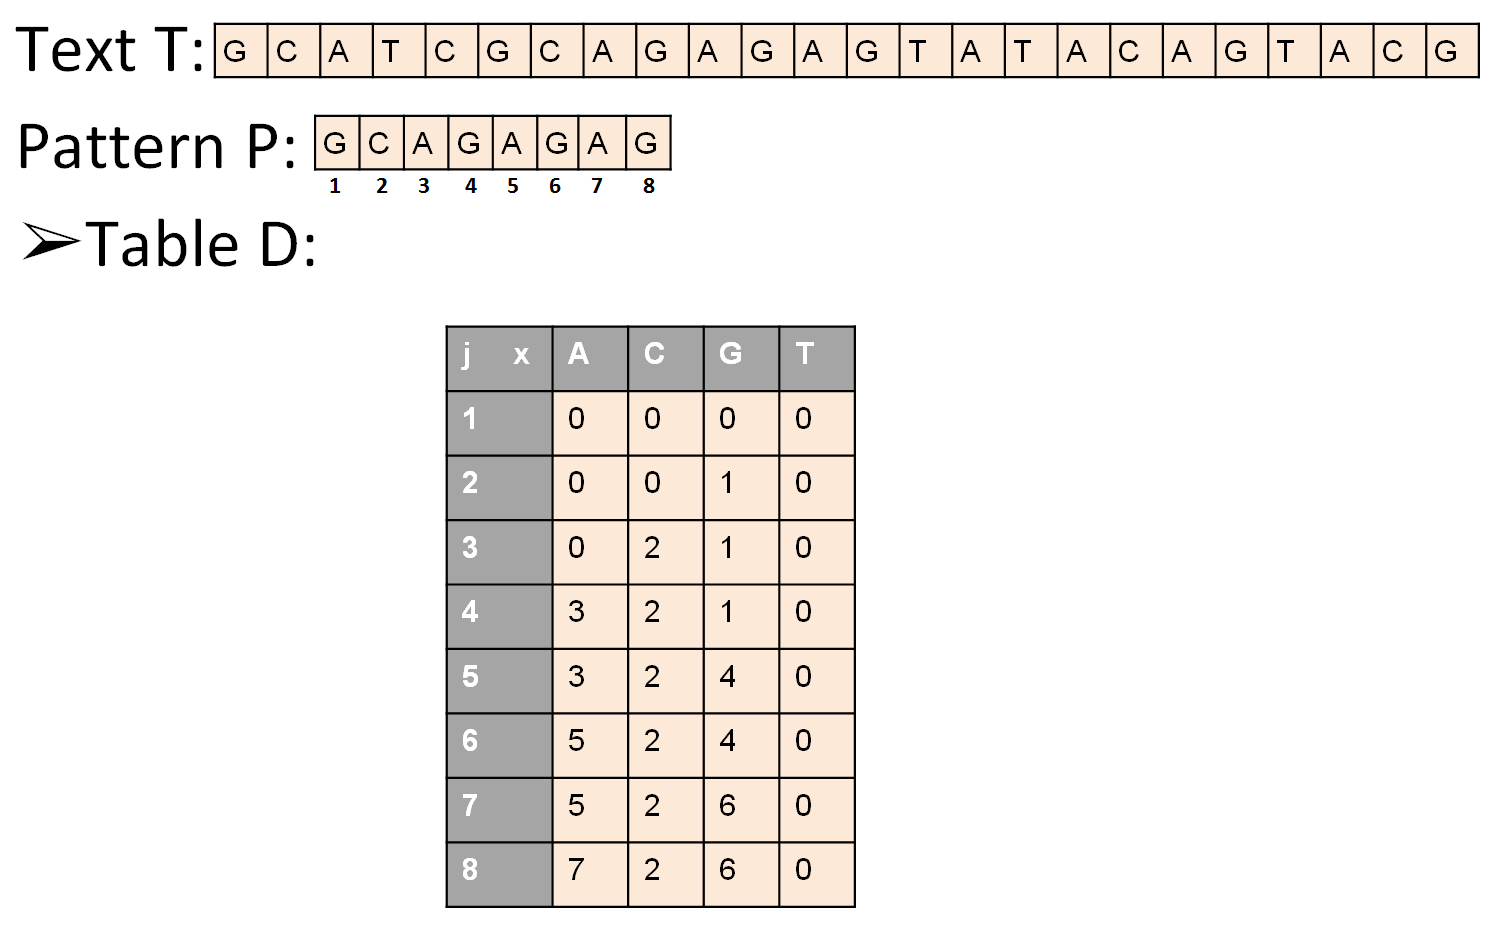
\includegraphics[width=0.8\textwidth]{figures/Example_Table.png}
\caption{Table of preprocessing phase}
\label{table}
\end{figure}

\subsection{Searching Phase}
In the searching phase, the algorithm needs shift the pattern and sequentially match it with the aligned text. Starting from the rightmost character in P, the algorithm checks the aligned character in T. If the pair of characters are matching, it sequentially continues the check to the next left character. If a mismatch occurs at position j in P, the algorithm needs to shift P according to the mismatched character in the text. For example, if at position j, the text contains a character that is not found in P, the pattern should be shifted by j. However, if the mismatched character is found in P, the pattern should be shifted by j-i, where i corresponds to the rightmost occurrence of this character in P. The index i of the last occurrence is retrieved from table D and i=D[j,x] where x is the character in the text. Figure \ref{search} shows the searching phase for the example shown in the previous section.

\begin{figure}[h!]
\centering
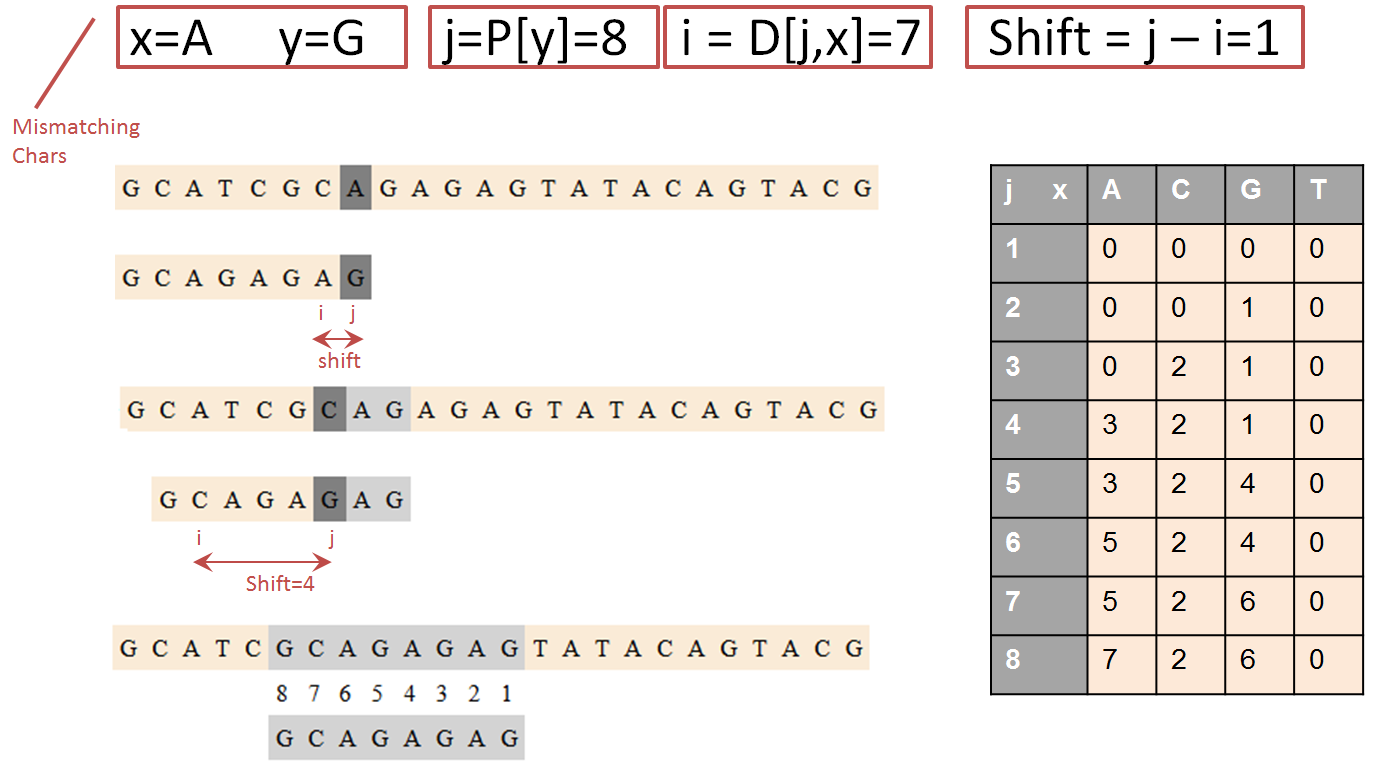
\includegraphics[width=0.8\textwidth]{figures/searching_phase.png}
\caption{Searching Phase}
\label{search}
\end{figure}

\subsection{complexity}

\newpage
\bibliography{references}{}
\nocite{*}

\end{document}
